\section*{Backup}

%%%%%%%%%%%%%%%%%%%%%%%%%%%%%%%%%%%%%%%%%%%%%%%%%%%%%%%%%%%%%%%%%%%%%%%%%%%%
\begin{frame}[noframenumbering]{}
    \vfill
    \centering
    \begin{beamercolorbox}[sep=8pt,center,shadow=true,rounded=true]{title}
        \usebeamerfont{section title}\NoHyper\insertsection\par\endNoHyper
    \end{beamercolorbox}
    \vfill
\end{frame}
%%%%%%%%%%%%%%%%%%%%%%%%%%%%%%%%%%%%%%%%%%%%%%%%%%%%%%%%%%%%%%%%%%%%%%%%%%%%
\begin{frame}[noframenumbering]{Software threats: Dynamic Information Flow Tracking}
    \begin{minipage}[c]{0.4\textwidth}
        \begin{block}{}
            \begin{itemize}
                \setbeamertemplate{itemize items}[square]
                \justifying
                \item Static or \underline{\textbf{Dynamic}}
                \item Software, \underline{\textbf{Hardware}} or Hybrid
            \end{itemize}
        \end{block}
    \end{minipage}\hfill%
    \begin{minipage}[c]{0.55\textwidth}
        \begin{figure}
            \centering
            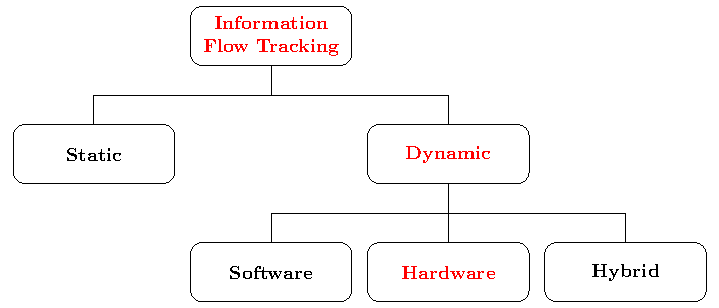
\includegraphics[width=\textwidth]{src/1_introduction/img/arborescence_ift.pdf}
            \caption{Taxonomy of IFTs}
            \label{fig:taxoDIFT}
        \end{figure}
    \end{minipage}
\end{frame}
%%%%%%%%%%%%%%%%%%%%%%%%%%%%%%%%%%%%%%%%%%%%%%%%%%%%%%%%%%%%%%%%%%%%%%%%%%%%
\begin{frame}[noframenumbering]{Tag Propagation Register}
    \begin{table}[!t]
        \centering
        \caption{Tag Propagation Register configuration}
        \label{tab:tpr}
        \resizebox{\linewidth}{!}{%
            \setlength{\tabcolsep}{2pt}
            \begin{tabular}{@{}lcccccccc@{}}
                \toprule
                          & Load/Store Enable & Load/Store Mode & Logical Mode & Comparison Mode & Shift Mode & Jump Mode & Branch Mode & Arith Mode \\ \cmidrule(lr){2-2}\cmidrule(lr){3-3}\cmidrule(lr){4-4}\cmidrule(lr){5-5}\cmidrule(lr){6-6}\cmidrule(lr){7-7}\cmidrule(lr){8-8}\cmidrule(lr){9-9}
                Bit index & 17 16 15          & 13 12           & 11 10        & 9 8             & 7 6        & 5 4       & 3 2         & 1 0        \\ \midrule
                Policy V1 & 0 0 1             & 1  0            & 1  0         & 0 0             & 1 0        & 1 0       & 0 0         & 1 0        \\
                Policy V2 & 1 1 1             & 1  0            & 1  0         & 1 0             & 1 0        & 1 0       & 1 0         & 1 0        \\ \bottomrule
            \end{tabular}
        }
    \end{table}

    \begin{itemize}
        \justifying
        \item A Mode field for each class of instructions, which specifies how to propagate the tags of the input operands to the output operand tag.
              \begin{itemize}
                  \justifying
                  \item the output tag keeps its old value (00);
                  \item the output tag is set to one, if both the input tags are set to one (01);
                  \item the output tag is set to one, if at least one input tag is set to one (10);
                  \item the output tag is set to zero (11).
              \end{itemize}
        \item The three bits in the L/S enable field allow the policy to enable the source, source-address, and destination-address tags, respectively
    \end{itemize}
\end{frame}

\begin{frame}[noframenumbering]{Tag Check Register}
    \begin{table}[!t]
        \centering
        \caption{Tag Check Register configuration}
        \label{tab:tcr}
        \resizebox{\linewidth}{!}{%
            \setlength{\tabcolsep}{2pt}
            \begin{tabular}{@{}lcccccccc@{}}
                \toprule
                          & Execute Check & Load/Store Check & Logical Check & Comparison Check & Shift Check & Jump Check & Branch Check & Arith Check \\\cmidrule(lr){2-2}\cmidrule(lr){3-3}\cmidrule(lr){4-4}\cmidrule(lr){5-5}\cmidrule(lr){6-6}\cmidrule(lr){7-7}\cmidrule(lr){8-8}\cmidrule(lr){9-9}
                Bit index & 21            & 20 19 18 17      & 16 15 14      & 13 12 11         & 10 9 8      & 7 6 5      & 4 3          & 2 1 0       \\ \midrule
                Policy V1 & 1             & 1 0 1 0          & 0 0 0         & 0 0 0            & 0 0 0       & 0 0 0      & 0 0          & 0 0 0       \\
                Policy V2 & 0             & 0 0 0 0          & 0 0 0         & 0 0 0            & 0 0 0       & 0 0 0      & 0 0          & 0 1 1       \\ \bottomrule
            \end{tabular}
        }
    \end{table}

    \begin{itemize}
        \justifying
        \item The tag-check rules restrict the operations that may be performed on tagged data. If the check bit for an operand tag is set to one and the corresponding tag is equal to one, an exception is raised.
              \begin{itemize}
                  \justifying
                  \item For all the classes except Load/Store, there are three tags to consider: first input, second input, and output tags
                  \item For the Load/Store class there are four tags to take into account: source-address, source, destination-address, and destination tags
                  \item the additional Execute Check field is associated with the program counter and specifies whether to raise a security exception when the program-counter tag is set to one
              \end{itemize}
    \end{itemize}
\end{frame}
%%%%%%%%%%%%%%%%%%%%%%%%%%%%%%%%%%%%%%%%%%%%%%%%%%%%%%%%%%%%%%%%%%%%%%%%%%%%
\begin{frame}[noframenumbering]{Case 1: Buffer Overflow}
    \begin{table}[H]
        \scriptsize
        \centering
        \caption{Logical fault injection simulation campaigns results for exhaustive multi-bits faults in one register at a given clock cycle}
        \label{tab:chap6_results_multi_bitflip_reg_bo}
        \setlength{\tabcolsep}{3pt}
        \begin{tabular}{@{}ccccccccccc@{}}
            \toprule
                                                               &                & Crash & Silent & Delay & Detection & \tableTwoLines{Detection \&}{Correction} & \tableTwoLines{Double Error}{Detection} & Success                                       & Total       & \tableTwoLines{Execution}{time (h:min)} \\\midrule
            \multirow{12}{*}{\tableTwoLines{Buffer}{Overflow}} & No protection  & 0     & 927    & 6     & --        & --                                       & --                                      & 3 {\tiny (0.32\%)}                            & 936         & 00:08                           \\
                                                               & Simple parity  & 0     & 498    & 0     & 498       & --                                       & --                                      & 0                                             & 996         & 00:14                           \\
                                                               & Hamming 1 & 0     & 0      & 20    & --        & 1962                                     & --                                      & 10 {\tiny (0.50\%)}                           & 1992        & 00:28                           \\
                                                               & Hamming 2 & 0     & 0      & 12    & --        & 2038                                     & --                                      & 14 {\tiny (0.68\%)}                           & 2064        & 00:32                           \\
                                                               & Hamming 3 & 0     & 0      & 12    & --        & 2352                                     & --                                      & 12 {\tiny (0.51\%)}                           & 2376        & 00:28                           \\
                                                               & Hamming 4 & 0     & 0      & 12    & --        & 2712                                     & --                                      & 12 {\tiny (0.44\%)}                           & 2736        & 00:35                           \\
                                                               & Hamming 5 & 0     & 0      & 12    & --        & 2976                                     & --                                      & 12 {\tiny (0.40\%)}                           & 3000        & 00:45                           \\
                                                               & SECDED 1       & 0     & 0      & 8     & --        & 1393                                     & 648                                     & 3 {\tiny (0.15\%)}                            & 2052        & 00:30                           \\
                                                               & SECDED 2       & 0     & 0      & 5     & --        & 1475                                     & 666                                     & 2 {\tiny (0.09\%)}                            & 2148        & 00:30                           \\
                                                               & SECDED 3       & 0     & 0      & 4     & --        & 1932                                     & 726                                     & 2 {\tiny (0.08\%)}                            & 2664        & 00:40                           \\
                                                               & SECDED 4       & 0     & 0      & 0     & --        & 2370                                     & 822                                     & 0                                             & 3192        & 00:45                           \\
                                                               & SECDED 5       & 0     & 0      & 0     & --        & 2670                                     & 798                                     & 0                                             & 3468        & 00:55                           \\
            \bottomrule
        \end{tabular}
    \end{table}
\end{frame}
%%%%%%%%%%%%%%%%%%%%%%%%%%%%%%%%%%%%%%%%%%%%%%%%%%%%%%%%%%%%%%%%%%%%%%%%%%%%
\begin{frame}[fragile, noframenumbering]{Case 2: WU-FTPd}
    \begin{itemize}
        \justifying
        \item The vulnerability is the use of an unchecked user input as the format string parameter in functions that perform formatting, e.g. printf()
        \item An attacker can use the format tokens, to write into arbitrary locations of memory, e.g. the return address of the function.
    \end{itemize}

    \centering
    \begin{minipage}[c]{\textwidth}
        \begin{lstlisting}[language=C,label=code:printfNFormat]
void echo(){
    int a;
    register int i asm("x8");
    a = i;
    printf("%224u%n%35u%n%253u%n%n", 1, (int*) (a-4), 1, (int*) (a-3), 1, (int*) (a-2), (int*) (a-1));
}\end{lstlisting}
    \end{minipage}
\end{frame}

\begin{frame}[noframenumbering]{Case 2: WU-FTPd}
    \begin{figure}
        \centering
        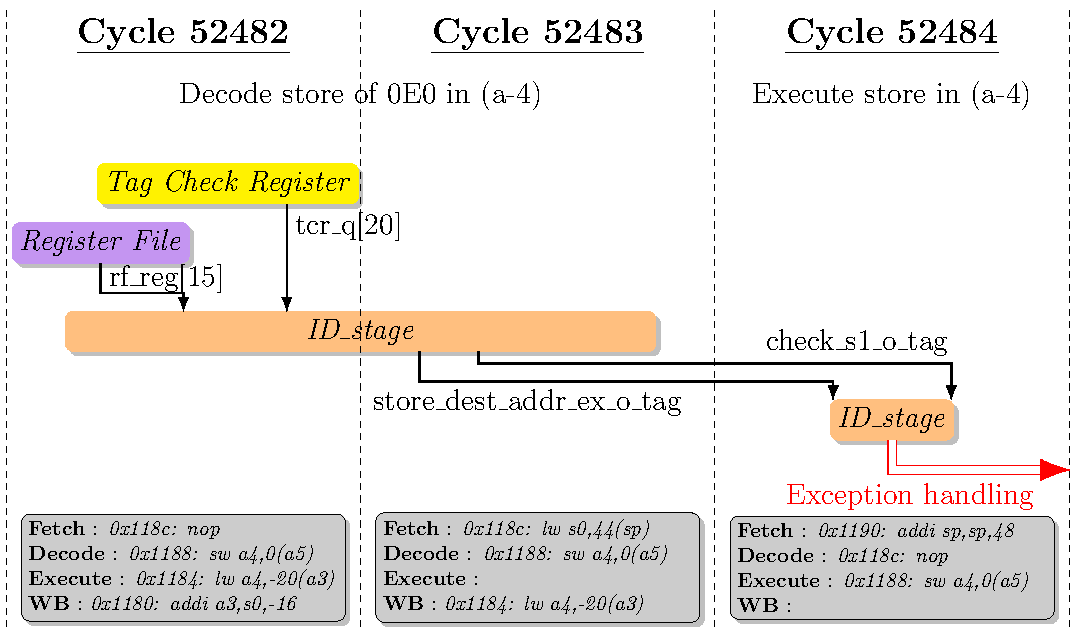
\includegraphics[height=.8\textheight]{src/2_vuln_assessment/img/wuftpd/ftpd_short.pdf}
        \caption{Temporal analysis of the tags propagation in a \textit{format string} attack}
        \label{fig:analyseTempoFormatString}
    \end{figure}
\end{frame}

\begin{frame}[noframenumbering]{Case 2: WU-FTPd}
    \begin{figure}
        \centering
        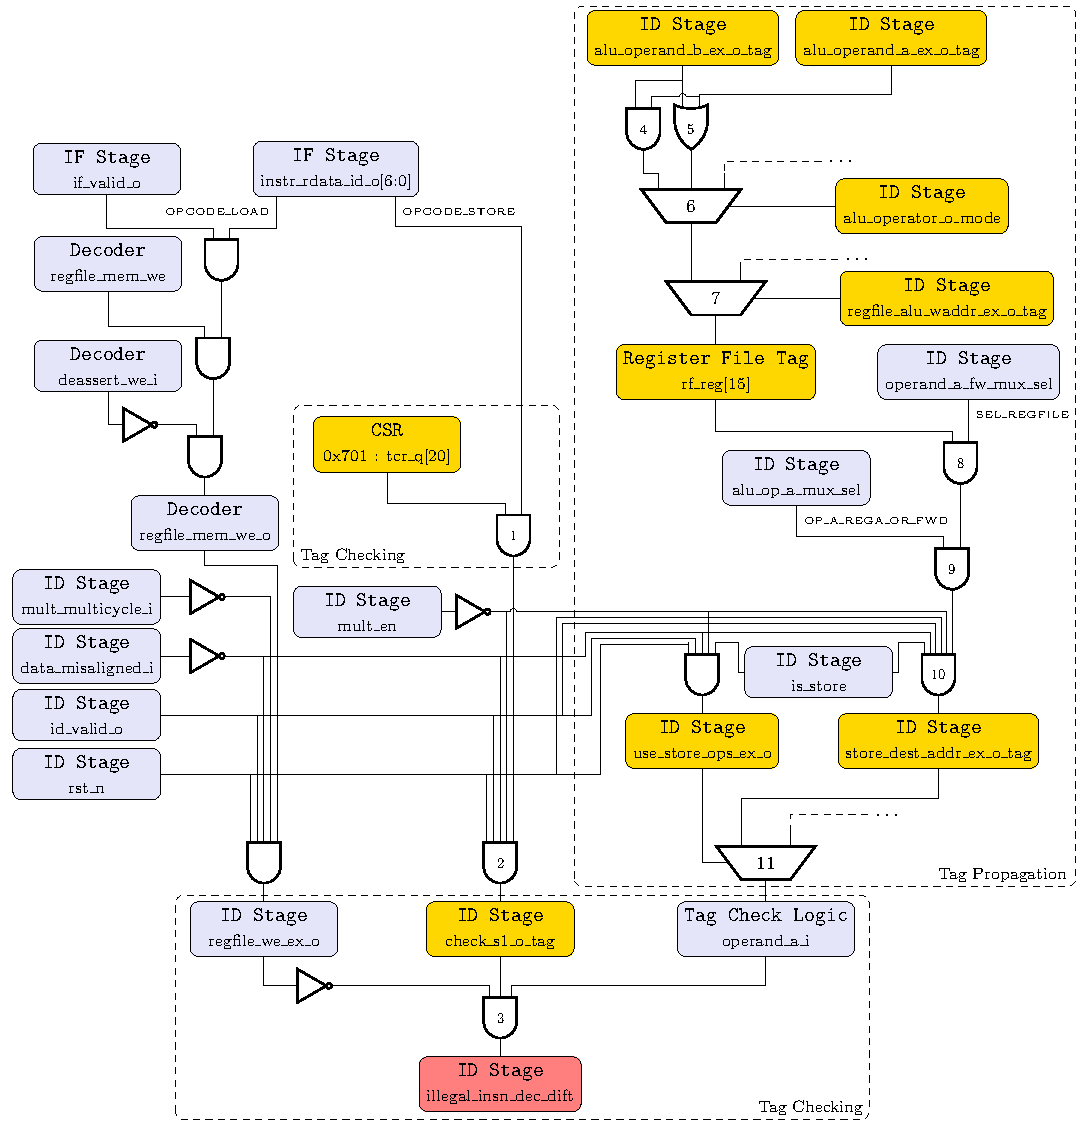
\includegraphics[height=.8\textheight]{src/2_vuln_assessment/img/wuftpd/arborescence_wuftpd.pdf}
        \caption{Logical analysis of the tags propagation in a \textit{format string} attack}
        \label{fig:analyseLogiqueFormatString}
    \end{figure}
\end{frame}

\begin{frame}[noframenumbering]{Case 2: WU-FTPd}
    \begin{table}[H]
        \scriptsize
        \centering
        \caption{Logical fault injection simulation campaigns results for single bit-flip in two registers at a given clock cycle}
        \label{tab:chap6_results_single_bitflip_spatial_fs}
        \setlength{\tabcolsep}{2pt}
        \begin{tabular}{@{}ccccccccccc@{}}
            \toprule
                                                             &               & Crash & Silent      & Delay      & Detection   & \tableTwoLines{Detection \&}{Correction} & \tableTwoLines{Double Error}{Detection} & Success                     & Total        & \tableTwoLines{Execution}{time (h:min)} \\\midrule
            \multirow{12}{*}{\tableTwoLines{Format}{String}} & No protection & 0     & \num{55589} & \num{5035} & --          & --                                       & --                                      & \num{3384} {\tiny (5.29\%)} & \num{64008}  & 163:09                                  \\
                                                             & Simple parity & 0     & \num{13361} & 450        & \num{54590} & --                                       & --                                      & 767  {\tiny (1.11\%)}       & \num{69168 } & 114:06                                  \\
                                                             & Hamming 1     & 0     & 0           & 1709       & --          & \num{89010 }                             & --                                      & 1089 {\tiny (1.19\%)}       & \num{91808 } & 179:38                                  \\
                                                             & Hamming 2     & 0     & 0           & 982        & --          & \num{96182 }                             & --                                      & 804  {\tiny (0.82\%)}       & \num{97968 } & 136:40                                  \\
                                                             & Hamming 3     & 0     & 0           & 659        & --          & \num{143883}                             & --                                      & 618  {\tiny (0.43\%)}       & \num{145160} & 261:40                                  \\
                                                             & Hamming 4     & 0     & 0           & 379        & --          & \num{206423}                             & --                                      & 222  {\tiny (0.11\%)}       & \num{207024} & 368:10                                  \\
                                                             & Hamming 5     & 0     & 0           & 391        & --          & \num{230758}                             & --                                      & 211  {\tiny (0.09\%)}       & \num{231360} & 445:58                                  \\
                                                             & SECDED 1      & 0     & 0           & 0          & --          & \num{82480 }                             & \num{15488}                             & 0                           & \num{97968 } & 233:28                                  \\
                                                             & SECDED 2      & 0     & 0           & 0          & --          & \num{92472 }                             & \num{14456}                             & 0                           & \num{106928} & 185:35                                  \\
                                                             & SECDED 3      & 0     & 0           & 0          & --          & \num{171168}                             & \num{12872}                             & 0                           & \num{184040} & 317:20                                  \\
                                                             & SECDED 4      & 0     & 0           & 0          & --          & \num{272080}                             & \num{9880 }                             & 0                           & \num{281960} & 462:58                                  \\
                                                             & SECDED 5      & 0     & \num{16128} & 0          & --          & \num{286296}                             & \num{10056}                             & 0                           & \num{312480} & 558:16                                  \\
            \bottomrule
        \end{tabular}
    \end{table}
\end{frame}

\begin{frame}[noframenumbering]{Case 2: WU-FTPd}
    \begin{table}[H]
        \scriptsize
        \centering
        \caption{Logical fault injection simulation campaigns results for exhaustive multi-bits faults in one register at a given clock cycle}
        \label{tab:chap6_results_multi_bitflip_reg_fs}
        \setlength{\tabcolsep}{3pt}
        \begin{tabular}{@{}ccccccccccc@{}}
            \toprule
                                                               &                & Crash & Silent & Delay & Detection & \tableTwoLines{Detection \&}{Correction} & \tableTwoLines{Double Error}{Detection} & Success                                       & Total       & \tableTwoLines{Execution}{time (h:min)} \\\midrule
            \multirow{12}{*}{\tableTwoLines{Format}{String}}   & No protection  & 0     & 1202   & 32    & --        & --                                       & --                                      & 14 {\tiny (1.12\%)}                           & 1248        & 01:24                           \\
                                                               & Simple parity  & 0     & 661    & 0     & 665       & --                                       & --                                      & 2  {\tiny (0.15\%)}                           & 1328        & 02:12                           \\
                                                               & Hamming 1 & 0     & 0      & 62    & --        & 2565                                     & --                                      & 29 {\tiny (1.09\%)}                           & 2656        & 04:24                           \\
                                                               & Hamming 2 & 0     & 0      & 53    & --        & 2666                                     & --                                      & 33 {\tiny (1.20\%)}                           & 2752        & 03:36                           \\
                                                               & Hamming 3 & 0     & 0      & 47    & --        & 3090                                     & --                                      & 31 {\tiny (0.98\%)}                           & 3168        & 03:55                           \\
                                                               & Hamming 4 & 0     & 0      & 47    & --        & 3570                                     & --                                      & 31 {\tiny (0.85\%)}                           & 3648        & 04:25                           \\
                                                               & Hamming 5 & 0     & 0      & 41    & --        & 3930                                     & --                                      & 29 {\tiny (0.73\%)}                           & 4000        & 05:18                           \\
                                                               & SECDED 1       & 0     & 0      & 22    & --        & 1832                                     & 864                                     & 18 {\tiny (0.66\%)}                           & 2736        & 03:30                           \\
                                                               & SECDED 2       & 0     & 0      & 14    & --        & 1938                                     & 894                                     & 18 {\tiny (0.63\%)}                           & 2864        & 03:48                           \\
                                                               & SECDED 3       & 0     & 0      & 10    & --        & 2560                                     & 968                                     & 14 {\tiny (0.39\%)}                           & 3552        & 04:42                           \\
                                                               & SECDED 4       & 0     & 0      & 5     & --        & 3146                                     & 1096                                    & 9  {\tiny (0.21\%)}                           & 4256        & 05:42                           \\
                                                               & SECDED 5       & 0     & 0      & 4     & --        & 3554                                     & 1064                                    & 2  {\tiny (0.04\%)}                           & 4624        & 06:30                           \\
            \bottomrule
        \end{tabular}
    \end{table}
\end{frame}

\begin{frame}[noframenumbering]{Case 2: WU-FTPd}
    \begin{table}[H]
        \scriptsize
        \centering
        \caption{Logical fault injection simulation campaigns results for exhaustive multi-bits faults in two registers at a given clock cycle}
        \label{tab:chap6_results_multi_bitflip_reg_multi_fs}
        \setlength{\tabcolsep}{1pt}
        \begin{tabular}{@{}ccccccccccc@{}}
            \toprule
                                                             &               & Crash & Silent      & Delay       & Detection   & \tableTwoLines{Detection \&}{Correction} & \tableTwoLines{Double Error}{Detection} & Success                      & Total          & \tableTwoLines{Execution}{time (h:min)} \\\midrule
            \multirow{12}{*}{\tableTwoLines{Format}{String}} & No protection & 0     & \num{84419} & 4836        & --          & --                                       & --                                      & 2009 {\tiny (2.20\%)}        & \num{91264 }   & 104:15                                  \\
                                                             & Simple parity & 0     & \num{32275} & 147         & \num{71198} & --                                       & --                                      & 444 {\tiny (0.43\%)}         & \num{104064}   & 138:40                                  \\
                                                             & Hamming 1     & 0     & 0           & \num{20050} & --          & \num{375836}                             & --                                      & 9234 {\tiny (2.28\%)}        & \num{405120}   & 902:08                                  \\
                                                             & Hamming 2     & 0     & 0           & \num{17597} & --          & \num{408894}                             & --                                      & \num{10757} {\tiny (2.46\%)} & \num{437248}   & 774:40                                  \\
                                                             & Hamming 3     & 0     & 0           & \num{17926} & --          & \num{564154}                             & --                                      & \num{11456} {\tiny (1.93\%)} & \num{593536}   & 1021:50                                 \\
                                                             & Hamming 4     & 0     & 0           & \num{20986} & --          & \num{767604}                             & --                                      & \num{13714} {\tiny (1.71\%)} & \num{802304}   & 1418:24                                 \\
                                                             & Hamming 5     & 0     & 0           & \num{20547} & --          & \num{934077}                             & --                                      & \num{14336} {\tiny (1.48\%)} & \num{968960}   & 1690:05                                 \\
                                                             & SECDED 1      & 0     & 0           & 5408        & --          & \num{194766}                             & \num{227655}                            & 4171 {\tiny (0.97\%)}        & \num{432000}   & 740:21                                  \\
                                                             & SECDED 2      & 0     & 0           & 3611        & --          & \num{220568}                             & \num{247704}                            & 4565 {\tiny (0.96\%)}        & \num{476448}   & 836:41                                  \\
                                                             & SECDED 3      & 0     & 0           & 3088        & --          & \num{395487}                             & \num{351553}                            & 4304 {\tiny (0.57\%)}        & \num{754432}   & 1305:36                                 \\
                                                             & SECDED 4      & 0     & 0           & 1939        & --          & \num{604649}                             & \num{491945}                            & 3515 {\tiny (0.32\%)}        & \num{1102048}  & 1915:20                                 \\
                                                             & SECDED 5      & 0     & 0           & 1938        & --          & \num{766527}                             & \num{535209}                            & 998 {\tiny (0.08\%)}         & \num{1304672}  & 2287:38                                 \\
            \bottomrule
        \end{tabular}
    \end{table}
\end{frame}
%%%%%%%%%%%%%%%%%%%%%%%%%%%%%%%%%%%%%%%%%%%%%%%%%%%%%%%%%%%%%%%%%%%%%%%%%%%%%%%%%%%%%%%%%%%%%%%%%%%%%%%%%%%%
\begin{frame}[fragile,noframenumbering]{Case 3: Compare/Compute}
    \begin{itemize}
        \justifying
        \item No software vulnerability
        \item Used to cover the DIFT surface
    \end{itemize}

    \centering
    \begin{minipage}[c]{\textwidth}
        \begin{lstlisting}[language=C,label=code:compareCompute]
int main(){
    int a, b = 5, c;
    register int reg asm("x9");
    a = reg;
    asm volatile("csrw 0x700, tprValue");
    asm volatile("csrw 0x701, tcrValue");
    asm volatile("p.spsw x0, 0(\%0);" :: "r" (&a));
    c = (a > b) ? (a-b) : (a+b);
        //42c:   ble a4,a5,448
        //430:   addi a5,s0,-16
        //434:   lw a4,-12(a5)
        //438:   addi a3,s0,-16
        //43c:   lw a5,-4(a3)
        //440:   sub a5,a4,a5
        //444:   j 45c
        //448:   addi a5,s0,-16
        //44c:   lw a4,-12(a5)
        //450:   addi a3,s0,-16
        //454:   lw a5,-4(a3)
        //458:   add a5,a4,a5
        //45c:   sw a5,-24(s0)
    return EXIT_SUCCESS;
}\end{lstlisting}
    \end{minipage}
\end{frame}

\begin{frame}[noframenumbering]{Case 3: Compare/Compute}
    \begin{figure}
        \centering
        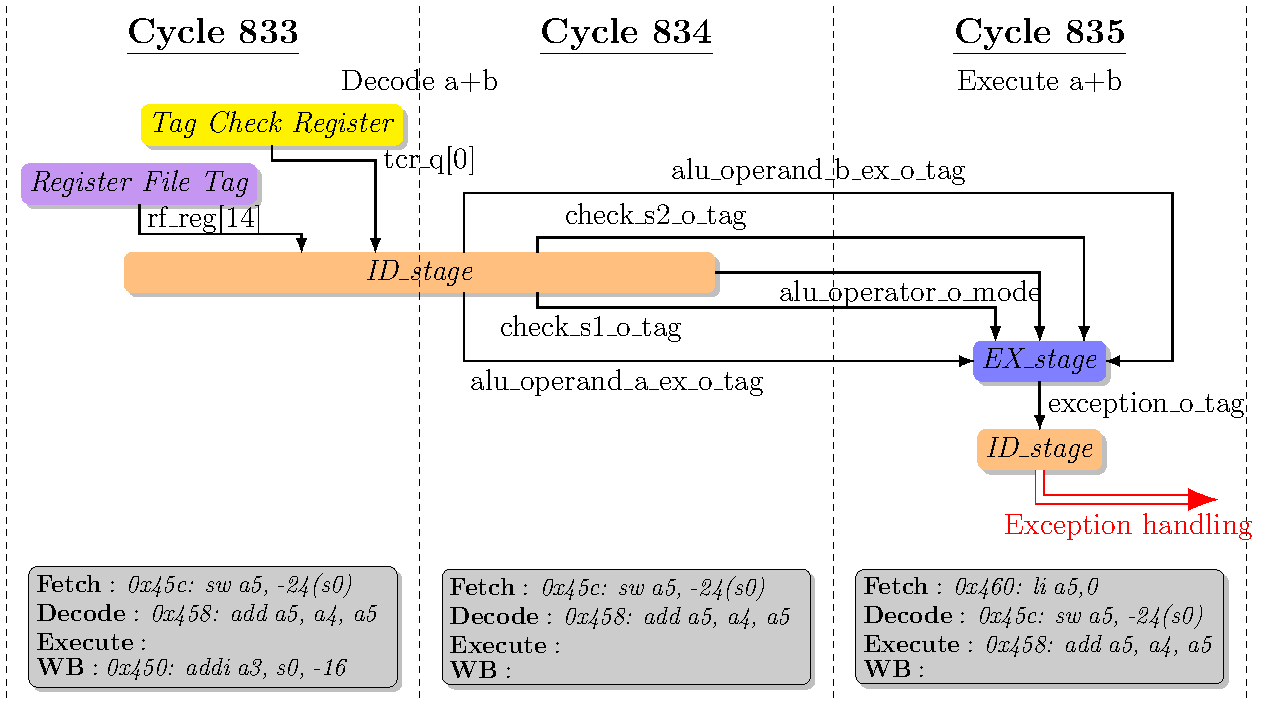
\includegraphics[height=.8\textheight]{src/2_vuln_assessment/img/comp_compu/attaquePropag_v3_short.pdf}
        \caption{Temporal analysis of the tags propagation in a \textit{format string} attack}
        \label{fig:analyseTempoCompCompute}
    \end{figure}
\end{frame}

\begin{frame}[noframenumbering]{Case 3: Compare/Compute}
    \begin{figure}
        \centering
        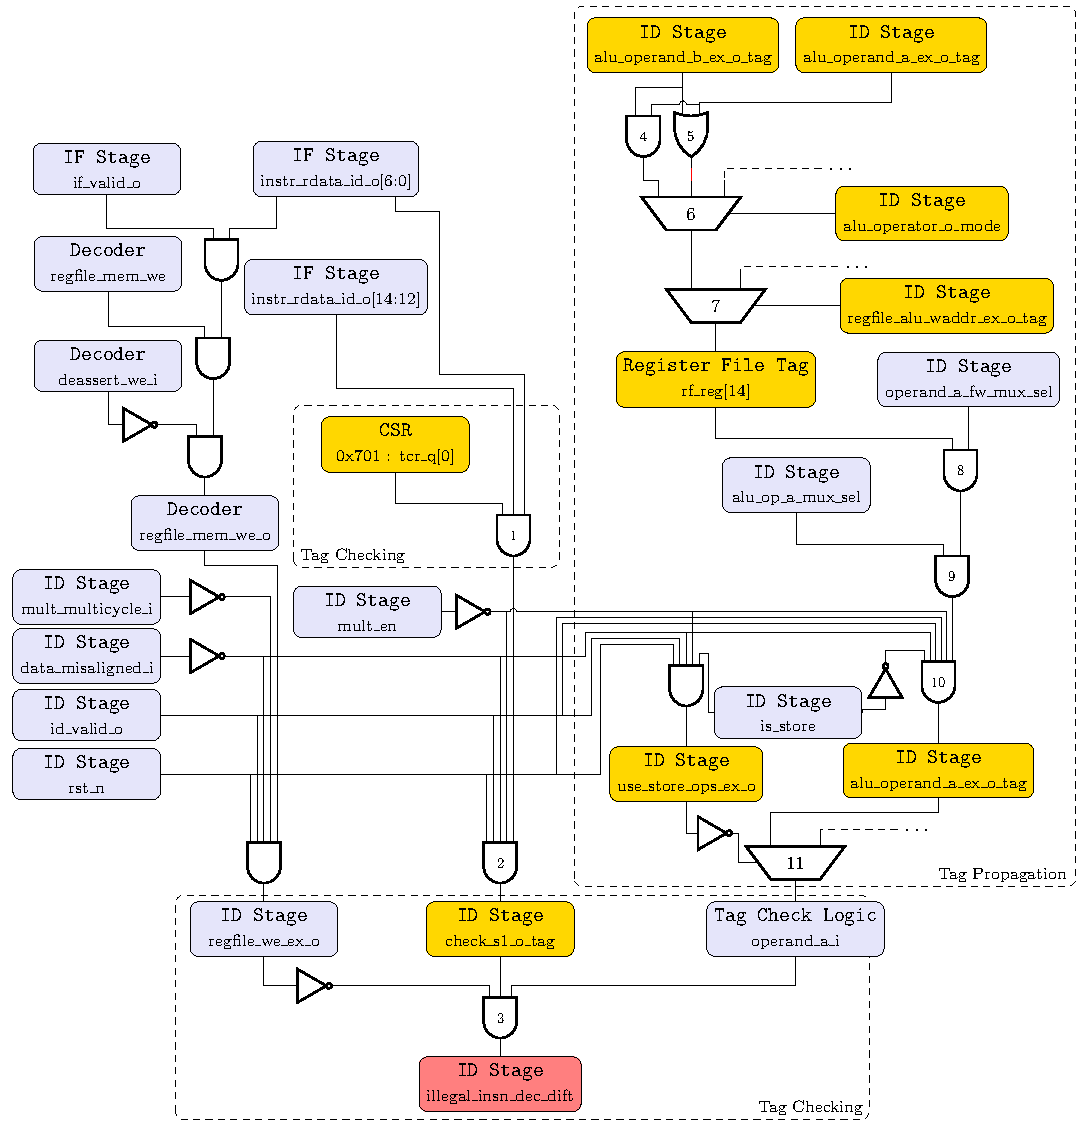
\includegraphics[height=.8\textheight]{src/2_vuln_assessment/img/comp_compu/arborescence_propagation.pdf}
        \caption{Logical analysis of the tags propagation in a \textit{format string} attack}
        \label{fig:analyseLogiqueCompCompute}
    \end{figure}
\end{frame}

\begin{frame}[noframenumbering]{Case 3: Compare/Compute}
    \begin{table}[H]
        \scriptsize
        \centering
        \caption{Logical fault injection simulation campaigns results for single bit-flip in two registers at a given clock cycle}
        \label{tab:chap6_results_single_bitflip_spatial_cc}
        \setlength{\tabcolsep}{2pt}
        \begin{tabular}{@{}ccccccccccc@{}}
            \toprule
                                                               &               & Crash & Silent      & Delay & Detection   & \tableTwoLines{Detection \&}{Correction} & \tableTwoLines{Double Error}{Detection} & Success                                              & Total         & \tableTwoLines{Execution}{time (h:min)} \\\midrule
            \multirow{12}{*}{\tableTwoLines{Compare}{Compute}} & No protection & 0     & \num{29906} & 919   & --          & --                                       & --                                      & \num{1179} {\tiny (3.68\%)}                          & \num{32004}   & 05:24                                   \\
                                                               & Simple parity & 0     & \num{6697}  & 202   & \num{27678} & --                                       & --                                      & 7   {\tiny (0.02\%)}                                 & \num{34584 }  & 04:48                                   \\
                                                               & Hamming 1     & 0     & 0           & 450   & --          & \num{45192  }                            & --                                      & 262 {\tiny (0.57\%)}                                 & \num{45904 }  & 09:21                                   \\
                                                               & Hamming 2     & 0     & 0           & 440   & --          & \num{48419  }                            & --                                      & 125 {\tiny (0.26\%)}                                 & \num{48984 }  & 08:47                                   \\
                                                               & Hamming 3     & 0     & 0           & 315   & --          & \num{72140  }                            & --                                      & 125 {\tiny (0.17\%)}                                 & \num{72580 }  & 13:53                                   \\
                                                               & Hamming 4     & 0     & 0           & 97    & --          & \num{103345 }                            & --                                      & 70  {\tiny (0.07\%)}                                 & \num{103512}  & 22:23                                   \\
                                                               & Hamming 5     & 0     & 0           & 96    & --          & \num{115511 }                            & --                                      & 73  {\tiny (0.06\%)}                                 & \num{115680}  & 23:48                                   \\
                                                               & SECDED 1      & 0     & 0           & 0     & --          & \num{37740  }                            & \num{11244}                             & 0                                                    & \num{48984 }  & 17:00                                   \\
                                                               & SECDED 2      & 0     & 0           & 0     & --          & \num{46236  }                            & \num{7228}                              & 0                                                    & \num{53464 }  & 10:12                                   \\
                                                               & SECDED 3      & 0     & 0           & 0     & --          & \num{85584  }                            & \num{6436}                              & 0                                                    & \num{92020 }  & 18:25                                   \\
                                                               & SECDED 4      & 0     & 0           & 0     & --          & \num{136040 }                            & \num{4940}                              & 0                                                    & \num{140980}  & 28:37                                   \\
                                                               & SECDED 5      & 0     & 0           & 0     & --          & \num{151212 }                            & \num{5028}                              & 0                                                    & \num{156240}  & 32:52                                   \\
            \bottomrule
        \end{tabular}
    \end{table}
\end{frame}

\begin{frame}[noframenumbering]{Case 3: Compare/Compute}
    \begin{table}[H]
        \scriptsize
        \centering
        \caption{Logical fault injection simulation campaigns results for exhaustive multi-bits faults in one register at a given clock cycle}
        \label{tab:chap6_results_multi_bitflip_reg_cc}
        \setlength{\tabcolsep}{3pt}
        \begin{tabular}{@{}ccccccccccc@{}}
            \toprule
                                                               &                & Crash & Silent & Delay & Detection & \tableTwoLines{Detection \&}{Correction} & \tableTwoLines{Double Error}{Detection} & Success                                       & Total       & \tableTwoLines{Execution}{time (h:min)} \\\midrule
            \multirow{12}{*}{\tableTwoLines{Compare}{Compute}} & No protection  & 0     & 616    & 2     & --        & --                                       & --                                      & 6  {\tiny (0.96\%)}                           & 624         & 00:04                           \\
                                                               & Simple parity  & 0     & 330    & 0     & 334       & --                                       & --                                      & 0                                             & 664         & 00:04                           \\
                                                               & Hamming 1 & 0     & 0      & 9     & --        & 1311                                     & --                                      & 8 {\tiny (0.60\%)}                            & 1328        & 00:09                           \\
                                                               & Hamming 2 & 0     & 0      & 15    & --        & 1356                                     & --                                      & 5 {\tiny (0.36\%)}                            & 1376        & 00:09                           \\
                                                               & Hamming 3 & 0     & 0      & 12    & --        & 1567                                     & --                                      & 5 {\tiny (0.32\%)}                            & 1584        & 00:11                           \\
                                                               & Hamming 4 & 0     & 0      & 12    & --        & 1807                                     & --                                      & 5 {\tiny (0.27\%)}                            & 1824        & 00:13                           \\
                                                               & Hamming 5 & 0     & 0      & 12    & --        & 1983                                     & --                                      & 5 {\tiny (0.25\%)}                            & 2000        & 00:14                           \\
                                                               & SECDED 1       & 0     & 0      & 2     & --        & 888                                      & 476                                     & 2 {\tiny (0.15\%)}                            & 1368        & 00:09                           \\
                                                               & SECDED 2       & 0     & 0      & 6     & --        & 977                                      & 449                                     & 0                                             & 1432        & 00:10                           \\
                                                               & SECDED 3       & 0     & 0      & 2     & --        & 1290                                     & 484                                     & 0                                             & 1776        & 00:12                           \\
                                                               & SECDED 4       & 0     & 0      & 0     & --        & 1580                                     & 548                                     & 0                                             & 2128        & 00:15                           \\
                                                               & SECDED 5       & 0     & 0      & 0     & --        & 1780                                     & 532                                     & 0                                             & 2312        & 00:16                           \\
            \bottomrule
        \end{tabular}
    \end{table}
\end{frame}

\begin{frame}[noframenumbering]{Case 3: Compare/Compute}
    \begin{table}[H]
        \scriptsize
        \centering
        \caption{Logical fault injection simulation campaigns results for exhaustive multi-bits faults in two registers at a given clock cycle}
        \label{tab:chap6_results_multi_bitflip_reg_multi_cc}
        \setlength{\tabcolsep}{1pt}
        \begin{tabular}{@{}ccccccccccc@{}}
            \toprule
                                                               &               & Crash & Silent      & Delay & Detection   & \tableTwoLines{Detection \&}{Correction} & \tableTwoLines{Double Error}{Detection} & Success               & Total        & \tableTwoLines{Execution}{time (h:min)} \\\midrule
            \multirow{12}{*}{\tableTwoLines{Compare}{Compute}} & No protection & 0     & \num{44444} & 323   & --          & --                                       & --                                      & 865 {\tiny (1.90\%)}  & \num{45632 } & 05:36                                   \\
                                                               & Simple parity & 0     & \num{16033} & 53    & \num{35943} & --                                       & --                                      & 3 {\tiny (0.01\%)}    & \num{52032 } & 08:05                                   \\
                                                               & Hamming 1     & 0     & 0           & 2912  & --          & \num{196958}                             & --                                      & 2690 {\tiny (1.33\%)} & \num{202560} & 34:17                                   \\
                                                               & Hamming 2     & 0     & 0           & 4677  & --          & \num{211969}                             & --                                      & 1978 {\tiny (0.90\%)} & \num{218624} & 37:24                                   \\
                                                               & Hamming 3     & 0     & 0           & 4377  & --          & \num{290302}                             & --                                      & 2089 {\tiny (0.70\%)} & \num{296768} & 53:50                                   \\
                                                               & Hamming 4     & 0     & 0           & 5282  & --          & \num{393423}                             & --                                      & 2447 {\tiny (0.61\%)} & \num{401152} & 74:31                                   \\
                                                               & Hamming 5     & 0     & 0           & 5829  & --          & \num{475987}                             & --                                      & 2664 {\tiny (0.55\%)} & \num{484480} & 94:21                                   \\
                                                               & SECDED 1      & 0     & 0           & 656   & --          & \num{92123 }                             & \num{122731}                            & 490 {\tiny (0.23\%)}  & \num{216000} & 35:42                                   \\
                                                               & SECDED 2      & 0     & 0           & 1452  & --          & \num{112110}                             & \num{124659}                            & 3 {\tiny (0.0013\%)}       & \num{238224} & 43:38                                   \\
                                                               & SECDED 3      & 0     & 0           & 640   & --          & \num{200702}                             & \num{175871}                            & 3 {\tiny (0.0008\%)}       & \num{377216} & 72:32                                   \\
                                                               & SECDED 4      & 0     & 0           & 68    & --          & \num{304920}                             & \num{246033}                            & 3 {\tiny (0.00054\%)}       & \num{551024} & 109:22                                  \\
                                                               & SECDED 5      & 0     & 0           & 96    & --          & \num{384572}                             & \num{267665}                            & 3 {\tiny (0.00046\%)}       & \num{652336} & 128:21                                  \\
            \bottomrule
        \end{tabular}
    \end{table}
\end{frame}
%%%%%%%%%%%%%%%%%%%%%%%%%%%%%%%%%%%%%%%%%%%%%%%%%%%%%%%%%%%%%%%%%%%%%%%%%%%%%%%%%%%%%%%%%%%%%%%%%%%%%%%%%%%%
\begin{frame}{Implemented strategies - details}
    \begin{table}[t]
        \centering
        \small
        \caption{Summary of DIFT-related protected registers -- taking SECDED}
        \label{tab:detail_strategies_group}
        \begin{tabular}{@{}cccccc@{}}
            \toprule
                       & \begin{tabular}[c]{@{}c@{}}Number of\\ protected bits\end{tabular} & \begin{tabular}[c]{@{}c@{}}Number of\\ redundancy bits\end{tabular} & \begin{tabular}[c]{@{}c@{}}Number of\\ parity bits\end{tabular} & \begin{tabular}[c]{@{}c@{}}Number of\\ bits\end{tabular} \\ \midrule
            Strategy 1 & 107                                                                & 25                                                                  & 5                                                               & 157                                                      \\
            Strategy 2 & 107                                                                & 30                                                                  & 7                                                               & 164                                                      \\
            Strategy 3 & 107                                                                & 64                                                                  & 24                                                              & 215                                                      \\
            Strategy 4 & 103                                                                & 101                                                                 & 38                                                              & 266                                                      \\
            Strategy 5 & 102                                                                & 114                                                                 & 39                                                              & 280                                                      \\
            \bottomrule
        \end{tabular}
    \end{table}
\end{frame}
%%%%%%%%%%%%%%%%%%%%%%%%%%%%%%%%%%%%%%%%%%%%%%%%%%%%%%%%%%%%%%%%%%%%%%%%%%%%%%%%%%%%%%%%%%%%%%%%%%%%%%%%%%%%